% This file is isea.tex.  It contains the formatting instructions for and acts as a template for submissions to ISEA 2015.  It is based on the ICCC  formats and instructions.  It uses the files isea.sty, isea.bst and isea.bib, the first two of which also borrow from AAAI IJCAI formats and instructions.
% Modified from ICCC.tex by B. Bogart

\documentclass[letterpaper]{article}
\usepackage{isea}
\usepackage[pdftex]{graphicx}
\usepackage{times}
\usepackage{helvet}
\usepackage{courier}
\usepackage{url}
\usepackage{verbatim}
\usepackage[numbers]{natbib}
\pdfinfo{
/Title Extend segment routing for another source routing protocol named RPL for Linux
/Author Alexander Aring, Stefan Schmidt, Michael Richardson}
% The file isea.sty is the style file for ISEA 2015 proceedings.
%
\title{Extend segment routing for another source routing protocol named RPL for Linux}
\author{Alexander Aring, Stefan Schmidt, Michael Richardson\\
Unemployed Hobbyist, Open Source Developer, Sandelman Software Works\\
Ottawa, Canada/Brunswick, Germany\\
alex.aring@gmail.com, stefan@datenfreihafen.org, mcr@sandelman.ca\\
\newline
\newline
}
\setcounter{secnumdepth}{0}

\begin{document}
\maketitle
\begin{abstract}
RPL \cite{RFC6550} is an IPv6 routing protocol for Low-Power and Lossy networks and becomes interested to use inside the IoT world.

There exists a lot of different open source Linux RPL implementations out there which are using RPL with storing mode only.
Storing mode means that the routes are propagated via ICMPv6 RPL messages and stored inside the routing table of the Linux kernel.

A new thing which was never possible before without a hackish way is to handle non-storing mode.
Non-storing mode is using source routing by adding header information \cite{RFC6554} instead storing routes inside the routing table.

This talk is about to show an approach how to implement RPL source routing for the kernel and offer the necessary configuration interface to the user space.
As implementation we will use rpld \cite{rpld} to show an example RPL implementation which will take use of such configuration interface to support non-storing mode.
As reference we will lookup the Linux segment routing implementation and try to extend the existing code with the needs of RPL non-storing mode.
This paper shows the approach to implement RPL source routing header as it was discussed at Netdevconf 2.1.
\end{abstract}

\section{Keywords}

Linux, IPv6, Low-Power and Lossy Networks, LLN, IPv6 Routing Protocol for Low-Power and Lossy Networks, RPL, Segment Routing, Source Routing

\section{Introduction}

RPL contains main two operation modes which are storing and non-storing mode.
As this is the main concern about the paper, this section will at first explain the differences between these modes.
At first we describe how RPL generates routes based on an example mesh topology.
Because RPL generates a tree like routing graph there exists upward routes as a route to the root node and downward routes as a route to child nodes.

\subsection{Topology}

In this paper we simplify RPL routing graph as a tree like structure with one parent and a list of children named DODAG (Destination-Oriented Directed Acyclic Graph).
Out of scope are other topologies like having multiple roots or floating roots, where the root node can be changed during runtime.
We want to keep the topology simple enough to first tackle the issue of non-storing mode inside GNU/Linux environment.

RPL avoids to use the IPv6 neighbor discovery all nexthop destination will use link-local addresses which are setup by stateless autoconfiguration.
In order to get basic RPL configuration the network is flooded with a DIO (DODAG Information Object) message.

\subsection{Upward Routes}

Each node, except the root node (DODAG root), maintains upward routes.
In both operation modes the upwards routes are stored inside the routing table.
This nexthop address is declared as parent (DODAG parent), because in view of the actual node the root can be reached over the parent, then the next parent, and so on...
All unknown destination addresses will be routed to the parent which finally reach the root node.
The root can act then as a RPL Border Routing and route packets to a different IPv6 network.

\paragraph{Parent Selection}

In case of multiple possible parents RPL provide mechanism for parent selection.
One which considered all parent selection up to the root node is MRHOF \cite{RFC6719}.
MRHOF consider the link quality between the node and their parents.
However this is out of scope of this document as basic parent selection can be considered a first come, first serve strategy when a DIO message arrived.

\subsection{Downward Routes}

In downward routes the operation mode can be different.
The downward routes are there to reach child nodes until leaf nodes from any parent or the root.
As mentioned earlier the operation mode can be storing or non-storing mode.
In this section we describe the difference of both operation modes.

\paragraph{Storing Mode}

In storing mode the downward routes are stored in {\bf all} nodes inside the routing table in their IPv6 stack instance like the upward routes.
Each nodes reports to his parent, decided before over parent selection, his reachable nodes over his children.
Therefore a DAO (Destination Advertisement Object) message will be send to his parent which contains all child nodes.
For that reason a DAO contains multiple RPL Target Options which contains each global-link address reached by specific link-local child address.
Started from the leaf each node will report it's parent their children and add their own address.

As result each nodes maintains a routing table in their IPv6 stack instance how every child in view of a specific node can be reached.
If the destination address isn't specified in the routing table the default route will route the packet to the root node.
No source routing is involved, the forwarding inside this RPL operation mode is handled by looking up the forwarding table only.

\paragraph{Non-Storing Mode}

In non-storing mode the nodes doesn't store any forwarding table information except one route for upward routes.
This effects that all packets will be routed to the root node of the network.
The root node will take use of source routing and adds, in any case that the destination address is part of the RPL network, a RPL source routing header as IPv6 extension header.
This source routing header has every nexthop to reach the final destination node inside the RPL network.
A RPL node sends for this case the DAO message not to it's parent, it will be directly routed to the root node.
Such DAO message will contain two options, the node node global-link address and it's parent link-local address.
The root node has a full topology overview of the RPL network and can reconstruct the segment link-local addresses to reach a specific child node.

\section{Example}

This section describes a example topology to show the information described in the previous sections.

\subsection{Topology}

\begin{figure}[h]
	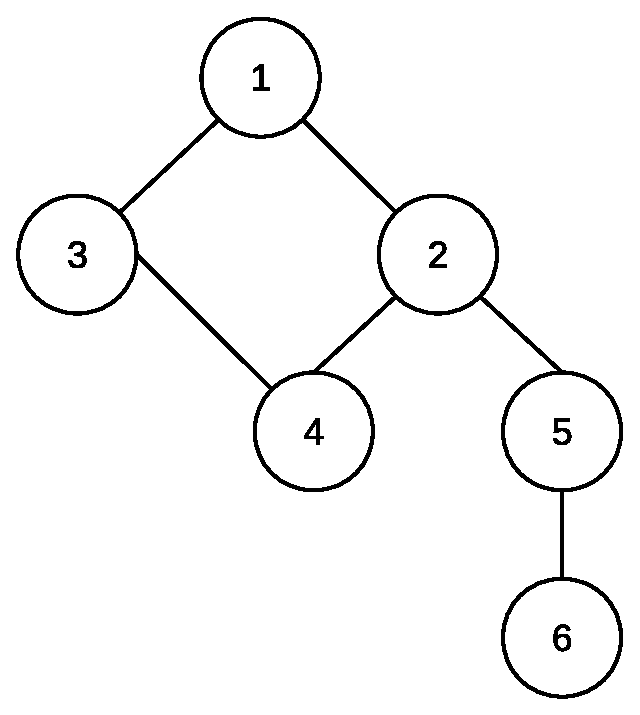
\includegraphics[width=3.31in]{figs/mesh0.eps}
	\caption{Example Mesh topology with bidirectional edges}
	\label{mesh0}
\end{figure}

Figure \ref{mesh0} shows a example mesh topology with bidirectional edges so every node can reach each other.
We will use this example topology to show a resulting RPL topology in ``storing-mode``.

\subsection{RPL DODAG}

\begin{figure}[h]
	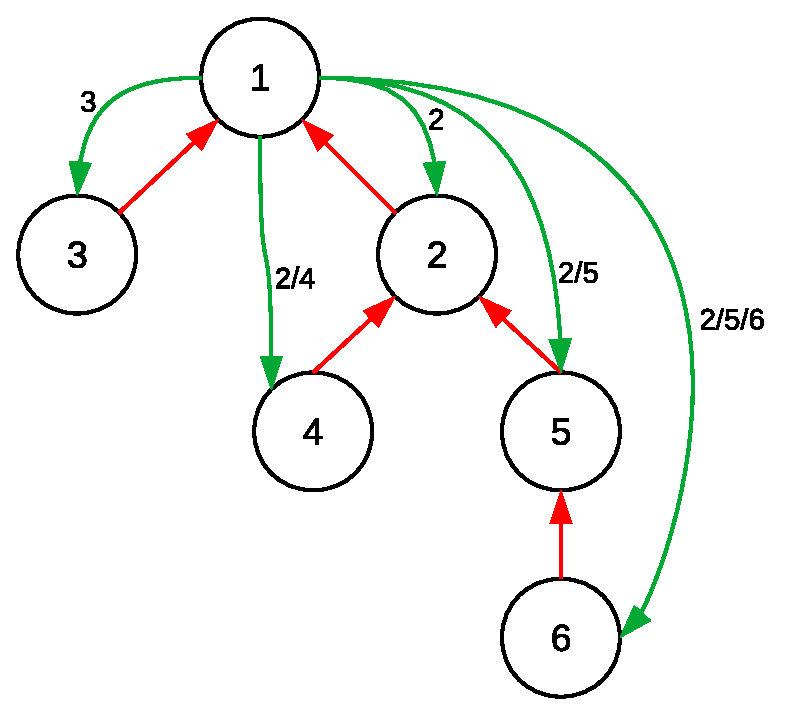
\includegraphics[width=3.31in]{figs/mesh1.eps}
	\caption{Resulting RPL topology in ``non-storing`` mode of mesh topology as shown in figure \ref{mesh0}}
	\label{mesh1}
\end{figure}

Figure \ref{mesh1} shows a possible resulting RPL DODAG of the mesh topology as shown in figure \ref{mesh0}.
Upward routes are shown as red directional arrows to reach the root node which was set by parent selection.
The root node stores a configuration to setup downward routes shown as green arrows.
These downward routes will be added as source routing header to the IPv6 header.
The children of the RPL network will actually not store any downard routes information and get the forwarding information from the routing header.
These forwarding information are shown beside the green arrows with node number and a separation character.
For example the root node can reach the child node 6 via node 2 over 5 to 6.

\section{Analysis}

At state of this document current RPL implementations for Linux like rpld or unstrung \cite{unstrung} are supporting storing mode only.
The reason why nobody implement non-storing mode so far is that there exists unsolved issues.
This section describes the problem in Linux which need to be solved to provide non-storing mode.
Afterwards multiple possible solution will be listed.
At the end a decision is made which will be the approach to provide non-storing mode under Linux.

\subsection{Problem}

The Problem is that IPv6 header generation is occurred inside the Linux kernel space.
As the RPL source routing header is an extension header of IPv6 header it need to be added inside the kernel transmit path of the IPv6 stack.
The current state of Linux kernel has no implementation to insert these headers to the IPv6 header.
Storing mode is not effected to this as it doesn't require the need of source routing.

On the receiving part, the IPv6 stack need to parse the RPL source header information and forward it to the nexthop if necessary.

\subsection{Requirements}

The root node of the RPL DODAG (DODAG root) need to have the possibility to insert a RPL source header with specific configurations per destination address.
This is necessary when a IPv6 packet from the childs arrived over it's parent path and need to be forwarded to another known child of the RPL network which only the root node knows.
If a root wants to send a packet to a known child the RPL source route header need to be attached with the right path information to it's child as well.

{\bf Each node} need to handle the RPL source routing header by parsing the header and handle forwarding of this packet to the nexthop correctly as RFC6554 describes.
This need to be done in the Linux IPv6 forwarding plane and not after.

\subsection{Socket Option}

There exists the possibility to add a specific source route header over the socket option ``IPV6\_RTHDR`` in Linux.
This can be used to place a RPL source routing header per IPv6 on a per socket setup.
It can be used to send out IPv6 packets with a specific RPL source header without getting the kernel involved of placing a source routing header.

The socket option cannot be used to implement to meet both requirements to add a specific source routing header for a specific destination address as it is only used inside the per socket context.
As well it cannot handle the parsing of IPv6 packets and forwarding them by not reaching the Linux socket layer.
This option likely made for doing experimental source routing header configuration and send them out.

\subsection{Lightweight Tunnel}

A lightweight tunnel (lwtunnel) in Linux can be used to meet the requirement of generating RPL source route header for a specific destination.
Therefore we can lookup the implementation of IPv6 segment routing \cite{srh} of the Linux kernel implementation.
Leightweight tunnels can be registered over a ops structure inside the Linux kernel.
Per route destination, which is in RPL only a full IPv6 address and not a prefix route, a encapsulation type can be given to assign the route to a specific lwtunnel.
Incoming and internal packets for a specific destination lwtunnel will be encapsulated by a RPL source routing header with a specific configuration given by the lwtunnel at creation time.

There is still an open requirement of parsing and forwarding packets which will be discussed in the next section.

\subsection{Forwarding}

This section describes a solution how to parse and forward a IPv6 packet with a RPL source routing header.
The following approach is identical how IPv6 segment routing \cite{srh} is solving the same requirement.

In this approach the source routing header handling and forwarding is just placed into the next header handling of the IPv6 stack.

\subsection{eBPF}

The Linux kernel has eBPF hooks for the lwtunnel implementation.
This means that the generation of RPL source route header can be implemented as a lwtunnel in eBPF.

There exists no eBPF hooks for the forwarding requirement which also requires to parse the header and interact with the IPv6 forwarding handling.

\subsection{Decision}

After thinking about all possible ways how to implement the requirements we doing as Netdevconf 2.1 discussed a similar approach like IPv6 segment routing implementation.
The socket option doesn't meet the requirements and the eBPF handling requires new hooks and for the lwtunnel additional user space handling to make it work.
The conclusion is to provide a in kernel lwtunnel implementation and extend the IPv6 extension header parsing with handling for RFC6554 RPL source routing header.

\section{Design}

This section describes the design for the upcoming implementation part.
It contains the explanation of the user view how to use the RPL source routing functionality.
This contains Sysfs and Netlink handling.
As side note the compression functionality of the RPL source routing handling will be described.

\subsection{Sysfs}

As the segment routing implementation by default the processing of RPL source routing headers is disabled.
The interface IPv6 Sysfs configuration will be extended to allow the processing of such headers.

\subsection{Compression}

The RPL source routing header of RFC6554 can be in a compressed format.
According to the IPv6 destination address the same prefix bytes can be elided.
A compression implementation follows a simple design of providing compress and uncompress functionality.
Any provided format can be converted into a different format according to the destination address context information.

In some cases it's necessary to change source routing header information which may available in a compressed format.
To avoid mistakes in the implementation the common approach to handle such changes as following process:

\begin{enumerate}
\item{Uncompress RPL source routing header}
\item{Change RPL source routing header information}
\item{Compress RPL source routing header again}
\end{enumerate}

This provides a simple modification of the segment addresses as these are available in a non-compressed format.

\subsection{Linux Kernel Netlink}

The Netlink API should be very simple as the existing segment routing implementation.
Segment routing is made in such way to provide the source routing header as binary data according to an IPv6 routing prefix.
The RPL source routing Netlink API should offer the same way as segment routing is doing.
For simplification of API the routing header will be accepted only in a uncompressed format.
This can also only be handled in an uncompressed format because if the routing prefix is giving as non full address the final destination address is available at runtime only.
One exception is if the routing prefix is a full IPv6 address prefix, which can avoid a compression during runtime.

\subsection{rpld}

The RPL daemon exchange ICMPv6 messages to setup necessary routing information.
As state of writing this paper the RPL daemon already supports storing mode functionality.
When the rpld daemon is starting it will setup the necessary sysfs entry settings to allow the forwarding of RPL source routing headers.
The RPL daemon will be extended to support non-storing mode by introducing a new configuration option named ``mode-of-operation``.
RFC 6550 describes ``mode-of-operation`` as a byte parameter for broadcasting routing protocol parameters through the network.
The root node of the RPL will initial flooding the network with these parameters inclusive the global-link IPv6 address.
When other nodes receiving these parameters they doing their upward routes by doing parent selection.
Over upward routes the nodes sending their parent and own global-link address to the root node of the RPL network.
The RPL root node constructs the RPL topology and setups the downward routes to each node by using the RPL source routing Netlink API.

\subsection{iproute2}

The iproute2 design follows all other lightweight tunnel mechanism.
This functionality is not necessary for making the rpld daemon work, but it is a different configuration tool to show or manipulate the current RPL source routing settings.

\section{Implementation}

This section describes the implementation part of the design. It contains the necessary changes inside the Linux kernel or user space software which was needed to implement RPL in ``non-storing`` mode.

\subsection{Linux kernel}

The Linux kernel will be extended to forwarding and generating RPL source routing header to an Linux IPv6 stack generated IPv6 packet.

\paragraph{Compression Helpers}

To provide RPL compression and decompression functionality the file ``net/ipv6/rpl.c`` was introduced.
This will be always build with the Linux IPv6 Stack implementation because of the possibility to might handle RPL source routing headers during runtime.
This is part of the forwarding handling.

The API of the helper functionality is the following:

\begin{itemize}
	\item{size\_t ipv6\_rpl\_srh\_alloc\_size(unsigned char n)}
	\item{ipv6\_rpl\_srh\_size(unsigned char n, unsigned char cmpri, unsigned char cmpre)}
	\item{void ipv6\_rpl\_srh\_decompress(struct ipv6\_rpl\_sr\_hdr *outhdr, const struct ipv6\_rpl\_sr\_hdr *inhdr, const struct in6\_addr *daddr, unsigned char n)}
	\item{void ipv6\_rpl\_srh\_compress(struct ipv6\_rpl\_sr\_hdr *outhdr, const struct ipv6\_rpl\_sr\_hdr *inhdr, const struct in6\_addr *daddr, unsigned char n)}
\end{itemize}

There are two size calculation functionality, ``ipv6\_rpl\_srh\_alloc\_size()`` should be used to get allocation size to decompress the RPL header.
This function will allocate worst case memory size for segments area according to n segments.
On the other hand ``ipv6\_rpl\_srh\_size()`` will return the size of a compressed header according to the number of n segments and RPL specific parameters ``cmpri`` and ``cmpre``.
This function can be used to validate the a RPL header before dereferencing it to buffer overflows.

The necessary parameters used in the helpers are described as following:

\begin{description}
	\item[cmpri]{The amount of prefix bytes of the segment addresses (except last one) which are the same of the actual used IPv6 destination address}
	\item[cmpre]{The amount of prefix bytes of the last segment address which are the same of the actual used IPv6 destination address}
	\item[n]{Number of segments inside the segment header, can be calculated by cmpri and cmpre}
	\item[outhdr]{Destination buffer for the compression or decompression of RPL header}
	\item[inhdr]{Source buffer for the compression or decompression of RPL header}
\end{description}

\paragraph{Forwarding}

The forwarding implementation will be inserted regarding to the Linux kernel file ``net/ipv6/exthdrs.c`` which is always build.
As base implementation the most code was took over from the IPv6 segment routing implementation.
RPL source routing processing mechanism requires additionally handling at some points.

As segment routing the IPv6 destination address need to be swapped with the segment address one, pointed out by the ``segment\_left`` field of the RPL source routing header.
To do this manipulation we do a decompression, manipulation and compression handling.
As the header size can result in a different size before than afterwards a full skb\_pull() of the extension header is necessary.

Another requirement is to detect for possible loops in the address segments.
It need to be checked that non assigned IPv6 address on the forwarding route appears separate inside the segments array.
To reach that another function ``int ipv6\_chk\_rpl\_srh\_loop(struct net *net, const struct in6\_addr *segs, unsigned char nsegs)`` was introduced inside ``net/ipv6/addrconf.c``.
This helper functionality returns one if any address occurs separated inside the segmented array, otherwise it will return zero.
The packet will dropped and a special ICMPv6 error messages will be generated as RFC 6554 descibes.

\paragraph{Leightweight Tunnel}

To generate IPv6 packets with a RPL source routing header in Linux a lightweight tunnel implementation was introduced.
This feature can be disabled or enabled during compile time with the ``IPV6\_RPL\_LWTUNNEL`` config entry.
The implementation of this functionality can be found in ``net/ipv6/rpl\_iptunnel.c``.

The initial code handles only inline extension header and not IP encapsulation.
Although IP encapsulation is handled in the forwarding code the current RPL lwtunnel implementation doesn't support to generate such packets.
The reason is that it is not yet clear in which cases and which other requirements are needed when a IP encapsulation is required.
Currently the ROLL working group tries to summary these requirements in a different draft \cite{I-D.ietf-roll-useofrplinfo}.

\subsection{iproute2}

The iproute2 implementation contains two basic functionality to create a routing configuration for adding a RPL source routing header for a specific IPv6 destination address.
Therefore the specific segments are need to given from the command line.
As well the current configuration can be dumped via iproute2.
The parsing and printing from and to command line can be shared between IPv6 segment routing and RPL segment routing code.
As indicator to specify a RPL source routing lwtunnel configuration the keyword ``rpl`` will be used.

Example: ``ip -n ns0 -6 route add 2001::3 encap rpl segs fe80::c8fe:beef:cafe:cafe,fe80::c8fe:beef:cafe:beef dev lowpan0``

\subsection{rpld}

To implement ``non-storing`` mode a tree data structure to represent the current RPL topology inside the root node is required.
A basic implementation with key value of the global-link address and their link-local address was added to the rpld implementation.
If a DAO messages arrived the source global-link address will be used to store the node into the tree according to it's parent from the parent selection algorithm.
Storing a node inside the topology will occur that a Netlink message is send to the kernel to setup a RPL source route.
With such a mechanism every node reports to the root node their parent and own address, the root node can calculate the path from the root to it's child and construct the necessary segments setup from the taken path.

\section{Testing}

This section describes how we tested the implementation and confirmed that it's actual working.

\subsection{mac802154\_hwsim}

For our testing we used mac802154\_hwsim driver and constructed a mesh topology.
At the end we had several IPv6 capable interfaces separated in their net namespace in a specific topology.

\subsection{wireshark}

Wireshark \cite{wireshark} was used to capture traffic on the IPv6 interface to confirm the RPL source router header was inserted.
At writing of this paper Wireshark was capable to dissect the RPL source routing header so it was easy to verify the compression algorithm to work correctly regarding to the Wireshark implementation.

\subsection{iputils}

Finally iputils \cite{iputils} was used for ping and traceroute to confirm that every node was addressable.
Traceroute was showing the upward and downward routes correctly, that the traffic inside the RPL network was going always over the root node.

\section{Future Work}

This paper shows how the basic RPL segment routing is implemented for the Linux kernel.
However there exists something to do which are to support new features or performance tweaks.

\subsection{Tweaks}

Currently the uncompressed RPL header is set with the set by using the Netlink API.
During runtime the RPL header gets decompressed because the full IPv6 destination address is known.
In case of that the lwtunnel routing prefix is in a form of a full IPv6 destination address we can do a compression at configuration time.
This tweak will remove the compression algorithm during runtime in hotpath situation.
Also to have a full address routing prefix is common thing in the RPL routing protocol.

\subsection{IP encapsulation}

As mentioned the creation of IP encapsulation for RPL lwtunnels is not supported yet.
The only mode is inline. The ROLL IETF working group try to define the cases of when using IP encapsulation \cite{I-D.ietf-roll-useofrplinfo}.
However it was not necessary to get RPL source routing running in a controlled network.
In cases of that the internet is in between of two RPL networks IP encapsulation may be required.

\subsection{Mixed Mode}

Michael Richardson pointed out that the ROLL IETF working group is working in a mixed mode of ``storing`` and ``non-storing`` mode.
As ``non-storing`` mode routes every traffic over the RPL root in can happen that direct downward routes can be shorter.
This feature doesn't require any change to the Linux RPL kernel functionality, but RPL routing daemons like rpld need to be updated to set routes differently.

\section{Bugs}

This section describes bugs which we detected while implementing and using the showed approach for RPL source routing for Linux.

\subsection{IPv6 Segment Routing}

To implement a lwtunnel we figured out that in ``struct lwtunnel\_state`` has a field named ``headroom`` which was set inside the IPv6 segment routing implementation.
As we adapted the code base from the IPv6 segment routing implementation as well, we figured out that setting this value with an IPv6 minimum MTU size interface makes problems.
After doing research and finding out that this field was introduced by the MPLS leightweight tunnel which operates before the IP layer.
As the Linux interface MTU is layer 3, this headroom value specifies the additional amount which is required before IPv6 such as MPLS.
In out environment on an IPv6 minimum MTU interface the IPv6 segment routing ``sendmsg()`` call will return in an error.
There is still a discussion going on what the ``headroom`` value really means. As it breaks 6LoWPAN interface for the RPL lwtunnel implementation it is set to zero.

\subsection{iputils - Traceroute}

Traceroute wasn't working in the first run.
After debugging Wireshark messages and the iputils traceroute code it came out that this implementation isn't dealing with the next header chain of IPv6 correctly.
A quick hack was made and a problem description was send to iputils as pull-request \cite{iputilspr}. However Michael Richardson pointed out that handling next headers correctly has it's own RFC \cite{RFC7045}.
It's still pending to make a clean solution so it's just not working for RPL source routing extension headers.

\bibliographystyle{isea}
\bibliography{isea}

\end{document}
